

\subsection{Results in voting}

COMMENT TURNOUT 

\begin{table}[h!]
    \centering
    \caption{Impact of refugee camp exposure on turnout}
    \resizebox{0.6\textwidth}{!}{\begingroup
\centering
\begin{tabular}{lcc}
   \toprule
                                 & Spillovers     & Control as 20-40km \\   
                                 & (1)            & (2)\\  
   \midrule 
   Within 1 km                   & 0.0197$^{***}$ & 0.0256$^{***}$\\   
                                 & (0.0025)       & (0.0031)\\   
   Ring 5                        & 0.0057$^{***}$ &   \\   
                                 & (0.0019)       &   \\   
   Ring 10                       & 0.0039$^{**}$  &   \\   
                                 & (0.0018)       &   \\   
   Ring 15                       & 0.0009         &   \\   
                                 & (0.0018)       &   \\   
   Ring 20                       & -0.0002        &   \\   
                                 & (0.0018)       &   \\   
   Ring 25                       & -0.0023        &   \\   
                                 & (0.0019)       &   \\   
   Ring 30                       & -0.0025        &   \\   
                                 & (0.0018)       &   \\   
    \\
   R$^2$                         & 0.517          & 0.566\\  
   Observations                  & 262,080        & 74,954\\  
    \\
   Municipality fixed effects & $\checkmark$   & $\checkmark$\\   
   Time-Reg fixed effects     & $\checkmark$   & $\checkmark$\\   
   \bottomrule
\end{tabular}
\par\endgroup
}
    \label{table:communist_results}
        \vspace{0.5em}
        \begin{minipage}{0.6\textwidth}
            \footnotesize
            Note: In the first column, we estimate \cref{equation:political}. In the second column, the control group are those within 20-40km.  Standard errors (SE) are clustered at the municipality level. *** p$<$0.01, ** p$<$0.05, * p$<$0.1.
        \end{minipage}
\end{table}

\begin{figure}[htbp]
  \centering
  \caption{Impact of Refugee Camp Exposure on turnout - ring estimations}
  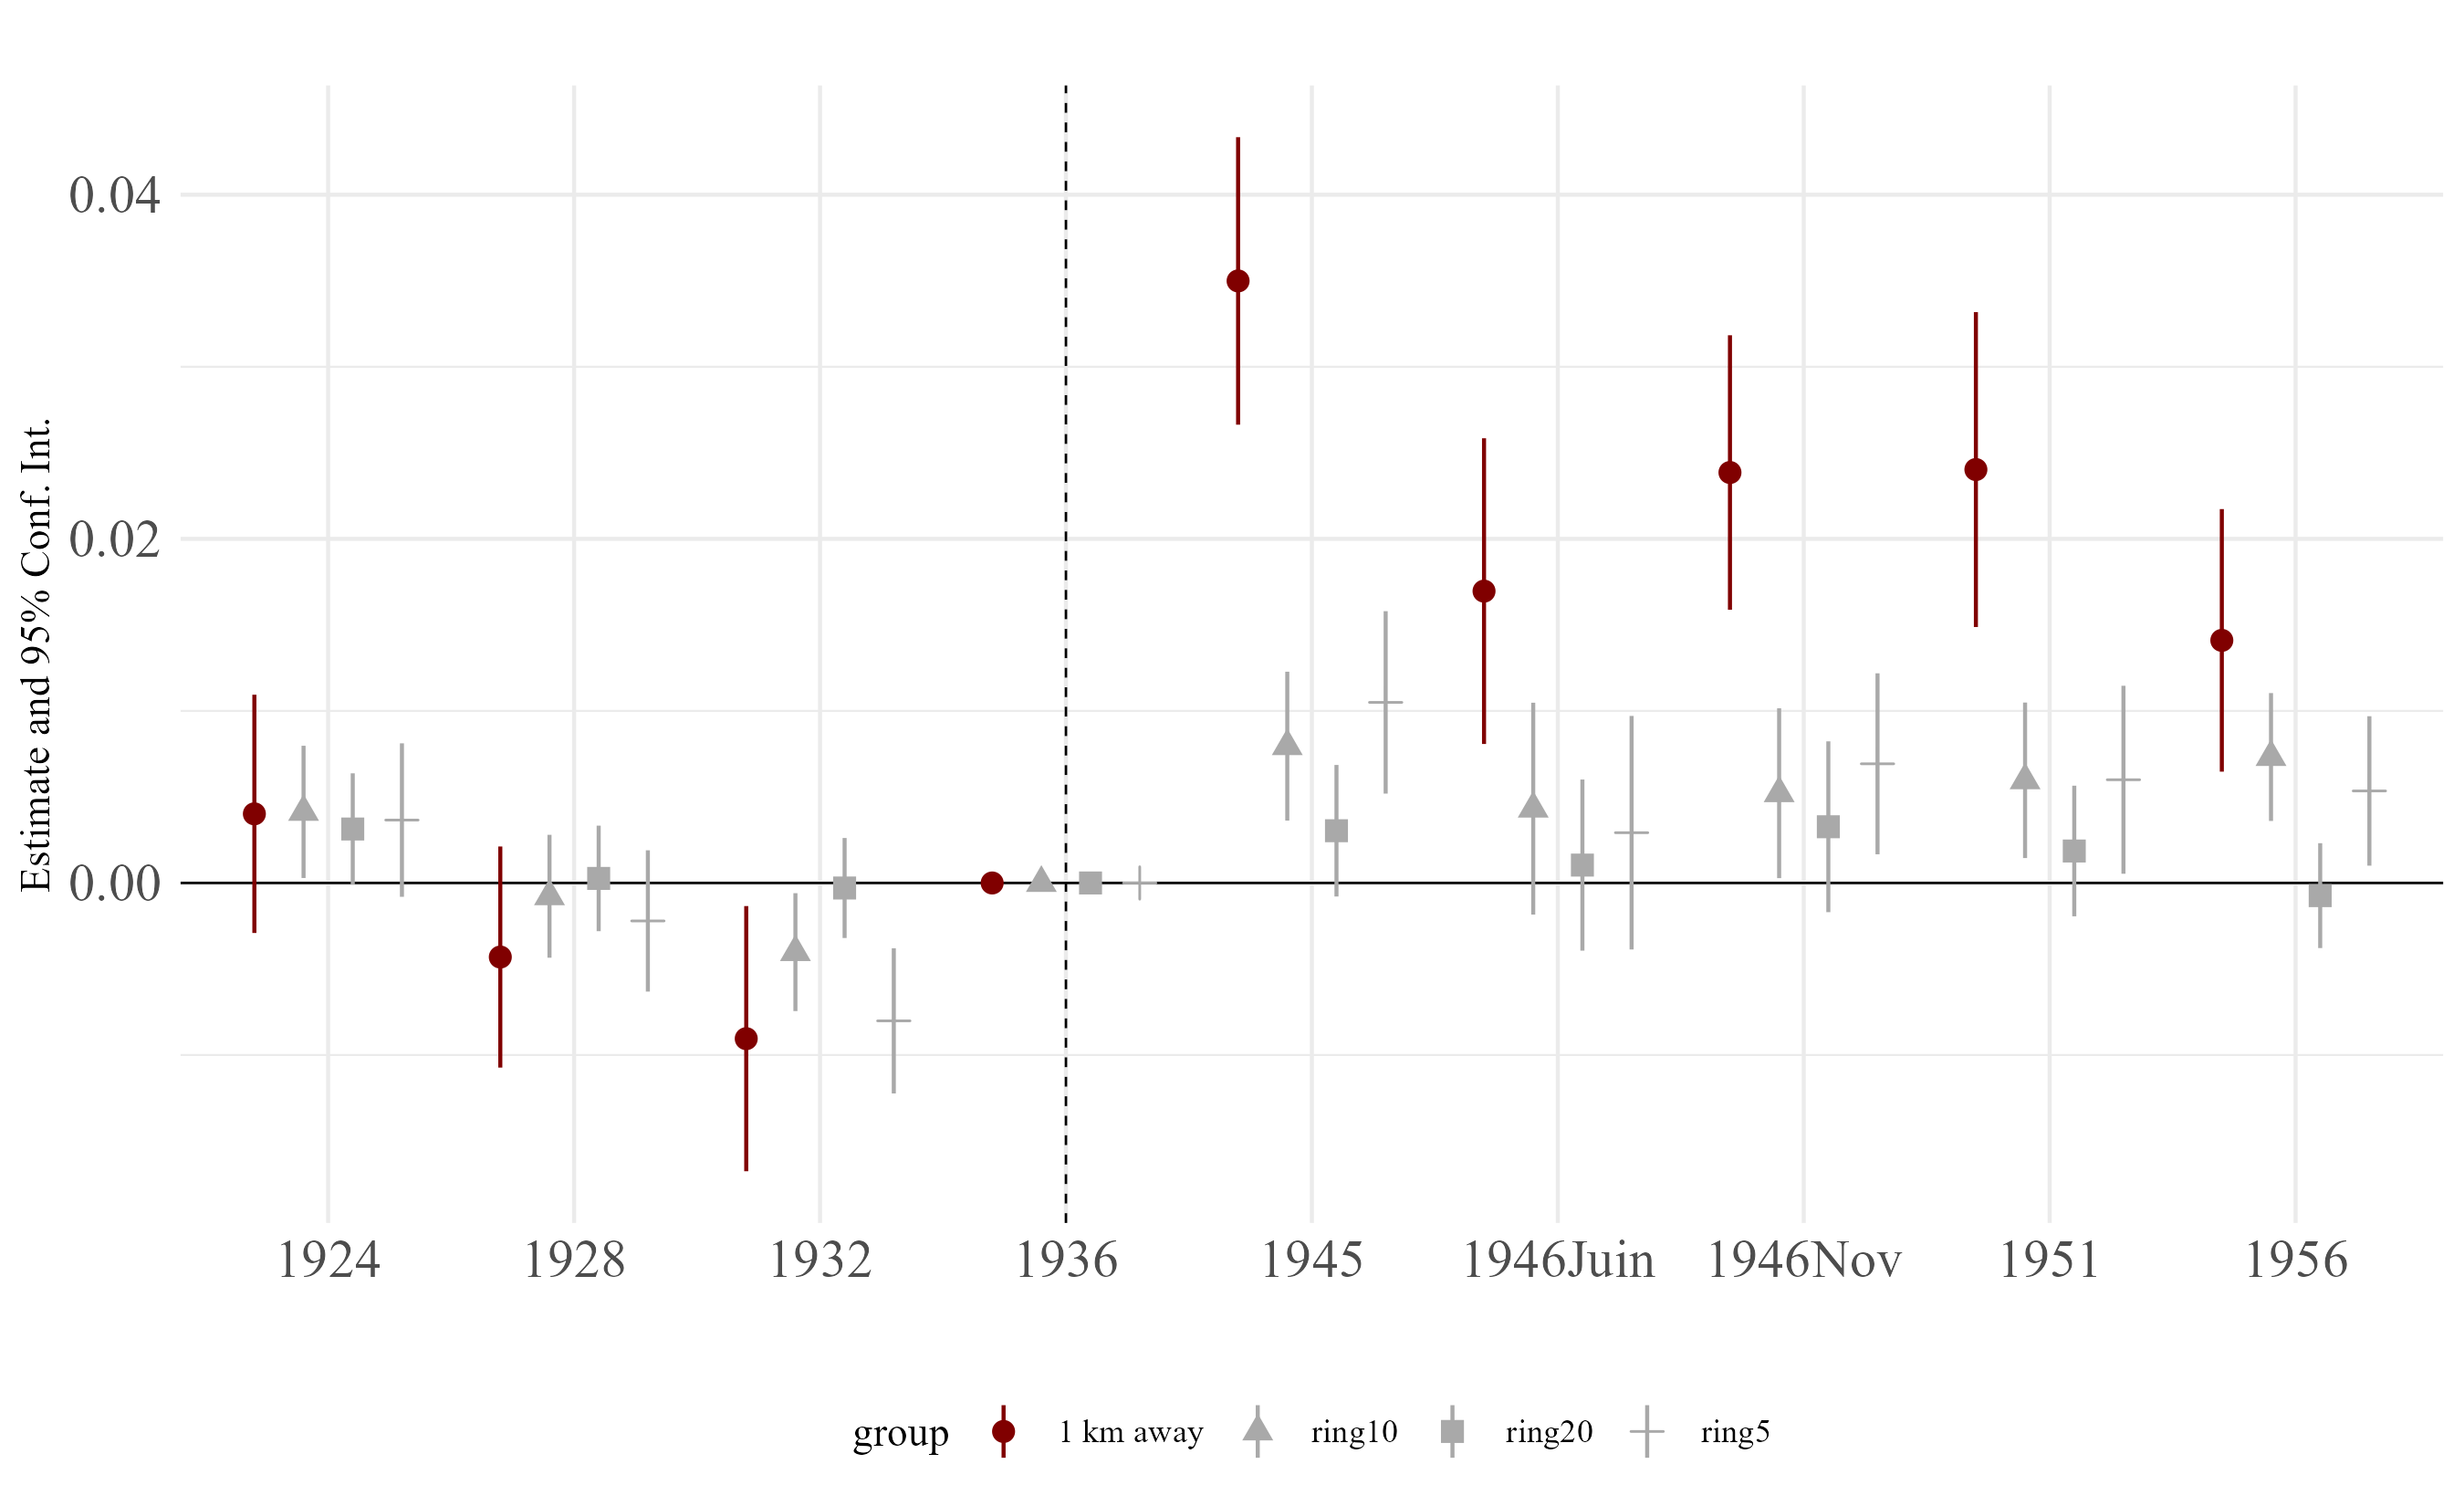
\includegraphics[width=0.8\linewidth]{figures/results/political/turnout_event_study.png}
  \label{fig:SFIO_all}
   \begin{minipage}{0.7\textwidth}
        \vspace{0.5em}
        {\footnotesize Notes: This graph reports the estimates from \cref{equation:political}, where the coefficient for each ring is estimated using municipalities located 20–40 km away as the control group. Error bars plot the interval confidence at 95\%. Standard errors are clustered at the municipality level.\par}
        \end{minipage}
\end{figure}


We examine how exposure to refugee camps affected political outcomes. The analysis focuses on the vote share of the SFIO (“Section Fran\c{c}aise de l’Internationale Ouvri`ere”), the socialist party, because it is the only political group that spans the entire period under study and it does not experience major ideological transformations before and after our treatment. \Cref{table:SFIO_results} shows several difference-in-differences specifications to examine the effect of hosting a camp on the share of votes of the socialist party. In the first column, we compare treated municipalities (those within 1 km) with cities within 40 km as controls. In the second column, we compare units treated units to those further away (within 20 to 40 km). The third column shows the coefficients of \Cref{equation:political}, which accounts for spatial spillovers by including a set of concentric circles. The results show a significant reduction in the share of votes for the socialist party in all the specifications. In our preferred specification, municipalities exposed to a camp have on average 2,7 percentage points lower vote share for the socialist party, which represents a 10\% reduction with respect to the pretreatment mean. 

\begin{table}[h!]
    \centering
    \caption{Impact of refugee camp exposure on socialist vote share}
    \resizebox{0.6\textwidth}{!}{\begingroup
\centering
\begin{tabular}{lcc}
   \toprule
                                 & Spillovers      & Control as 20-40km \\   
                                 & (1)             & (2)\\  
   \midrule 
   Within 1 km                   & -0.0150$^{***}$ & -0.0283$^{***}$\\   
                                 & (0.0038)        & (0.0055)\\   
   Ring 5                        & -0.0064$^{**}$  &   \\   
                                 & (0.0030)        &   \\   
   Ring 10                       & -0.0029         &   \\   
                                 & (0.0029)        &   \\   
   Ring 15                       & -0.0038         &   \\   
                                 & (0.0029)        &   \\   
   Ring 20                       & 0.0019          &   \\   
                                 & (0.0028)        &   \\   
   Ring 25                       & 0.0068$^{**}$   &   \\   
                                 & (0.0028)        &   \\   
   Ring 30                       & 0.0017          &   \\   
                                 & (0.0029)        &   \\   
    \\
   R$^2$                         & 0.779           & 0.789\\  
   Observations                  & 261,841         & 74,781\\  
    \\
   Municipality fixed effects & $\checkmark$    & $\checkmark$\\   
   Time-Reg fixed effects     & $\checkmark$    & $\checkmark$\\   
   \bottomrule
\end{tabular}
\par\endgroup
}
    \label{table:SFIO_results}
        \begin{minipage}{0.6\textwidth}
        \vspace{0.5em}
            \footnotesize
            Note: In the first column, we estimate \cref{equation:political}. In the second column, the control group are those within 20-40km.  Standard errors (SE) are clustered at the municipality level. *** p$<$0.01, ** p$<$0.05, * p$<$0.1.
        \end{minipage}
\end{table}

\Cref{fig:SFIO_all} shows the results of the event study by buffer size - within 1 km, within 10 km away and 20 km - considering the municipalities within 40 km as control group. Before the war, the coefficients suggest no systematic pre-trend for the estimations of municipalities that are nearby camps. After 1945, however, municipalities exposed to refugee camps record a persistent decline in SFIO support, with estimates becoming increasingly negative through the 1950s. This pattern is consistent with a political backlash: exposure to the camps may have deteriorated the image of the socialist left, historically associated with solidarity and internationalism, eroding their electoral support. The figure also shows significant spillovers effects to nearby municipalities. For municipalities within 30 km, the effects vanish because the buffer increasingly draws in control municipalities. 


\begin{figure}[htbp]
  \centering
  \caption{Impact of Refugee Camp Exposure on socialist vote share - ring estimations}
  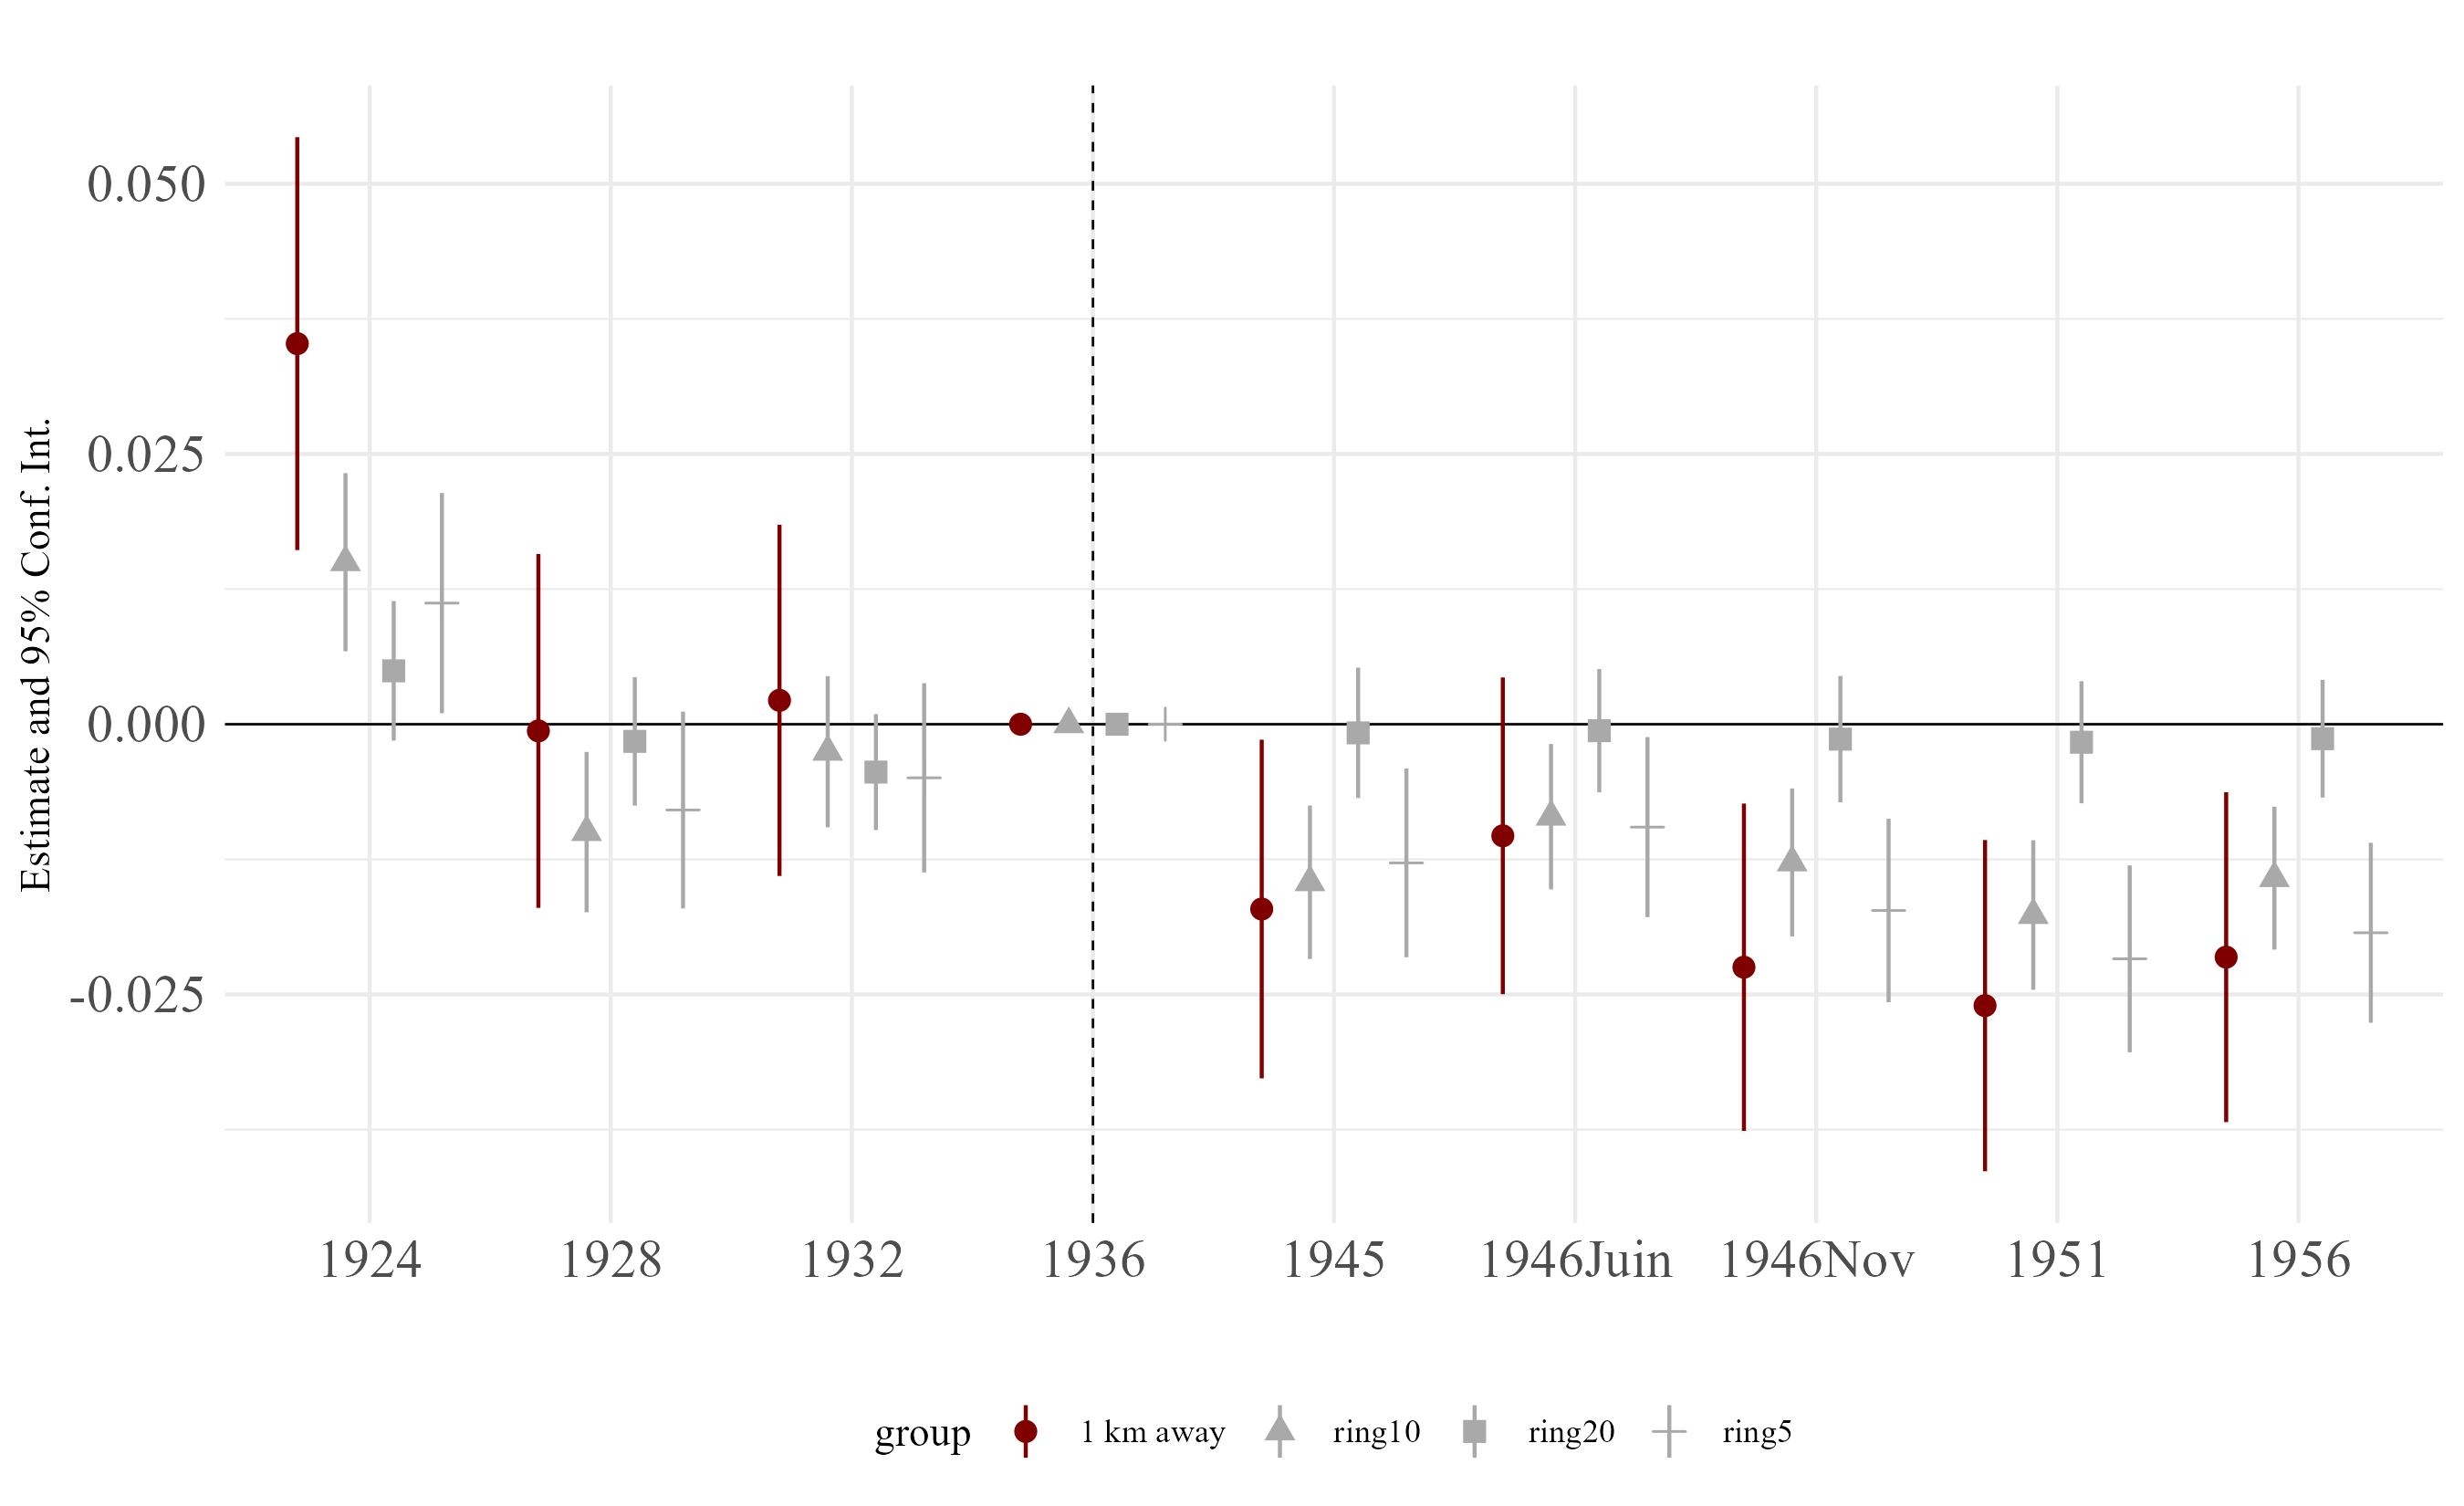
\includegraphics[width=0.8\linewidth]{figures/results/political/pvoixSFIO_event_study.png}
  \label{fig:SFIO_all}
   \begin{minipage}{0.7\textwidth}
        \vspace{0.5em}
        {\footnotesize Notes: This graph reports the estimates from \cref{equation:political}, where the coefficient for each ring is estimated using municipalities located 20–40 km away as the control group. Error bars plot the interval confidence at 95\%. Standard errors are clustered at the municipality level.\par}
        \end{minipage}
\end{figure}


Right-wing parties are not comparable before and after the shock because there is no single party that exists continuously throughout the entire period of analysis.\footnote{Throughout the interwar and post-war years, the composition of the French right changed substantially. Key parties present before the war—such as the Fédération républicaine or the Alliance démocratique—either disappeared, were absorbed, or were replaced after 1945 by entirely new formations like the MRP or, later, the Gaullist RPF.} We include the results on right-wing support in the Annex using the aggregation done by \citet{piketty_histoire_2023}, which shows a positive and significant effect, in line with our main results. 


\Cref{table:communist_results} extends this analysis by examining responses at the far left of the spectrum, focusing on the Communist Party. Because the PCF first appears in the 1924 legislative elections, caution is required due to limited pre-treatment periods. Nonetheless, once spatial spillovers are accounted for, we find that exposure to the camps increases the PCF vote share: municipalities within 1 km record an increase of roughly 1.6 percentage points or 15\% increase with respect to the pretreatment mean. The effects gradually decline toward zero as distance increases. 


\begin{table}[h!]
    \centering
    \caption{Impact of refugee camp exposure the communist vote shares}
    \resizebox{0.6\textwidth}{!}{\begingroup
\centering
\begin{tabular}{lcc}
   \toprule
                                 & Spillovers     & Control as 20-40km \\   
                                 & (1)            & (2)\\  
   \midrule 
   Within 1 km                   & 0.0166$^{***}$ & 0.0238$^{***}$\\   
                                 & (0.0033)       & (0.0050)\\   
   Ring 5                        & 0.0175$^{***}$ &   \\   
                                 & (0.0027)       &   \\   
   Ring 10                       & 0.0140$^{***}$ &   \\   
                                 & (0.0026)       &   \\   
   Ring 15                       & 0.0131$^{***}$ &   \\   
                                 & (0.0025)       &   \\   
   Ring 20                       & 0.0104$^{***}$ &   \\   
                                 & (0.0025)       &   \\   
   Ring 25                       & 0.0048$^{*}$   &   \\   
                                 & (0.0025)       &   \\   
   Ring 30                       & -0.0018        &   \\   
                                 & (0.0025)       &   \\   
    \\
   R$^2$                         & 0.823          & 0.831\\  
   Observations                  & 261,841        & 74,781\\  
    \\
   Municipality fixed effects & $\checkmark$   & $\checkmark$\\   
   Time-Reg fixed effects     & $\checkmark$   & $\checkmark$\\   
   \bottomrule
\end{tabular}
\par\endgroup
}
    \label{table:communist_results}
    \vspace{0.5em}
        \begin{minipage}{0.6\textwidth}
            \footnotesize
            Note: In the first column, we estimate \cref{equation:political}. In the second column, the control group are those within 20-40km.  Standard errors (SE) are clustered at the municipality level. *** p$<$0.01, ** p$<$0.05, * p$<$0.1.
        \end{minipage}
\end{table}

COMMENT EVENT STUDY 

\begin{figure}[htbp]
  \centering
  \caption{Impact of refugee camp exposure the communist vote shares - ring estimations}
  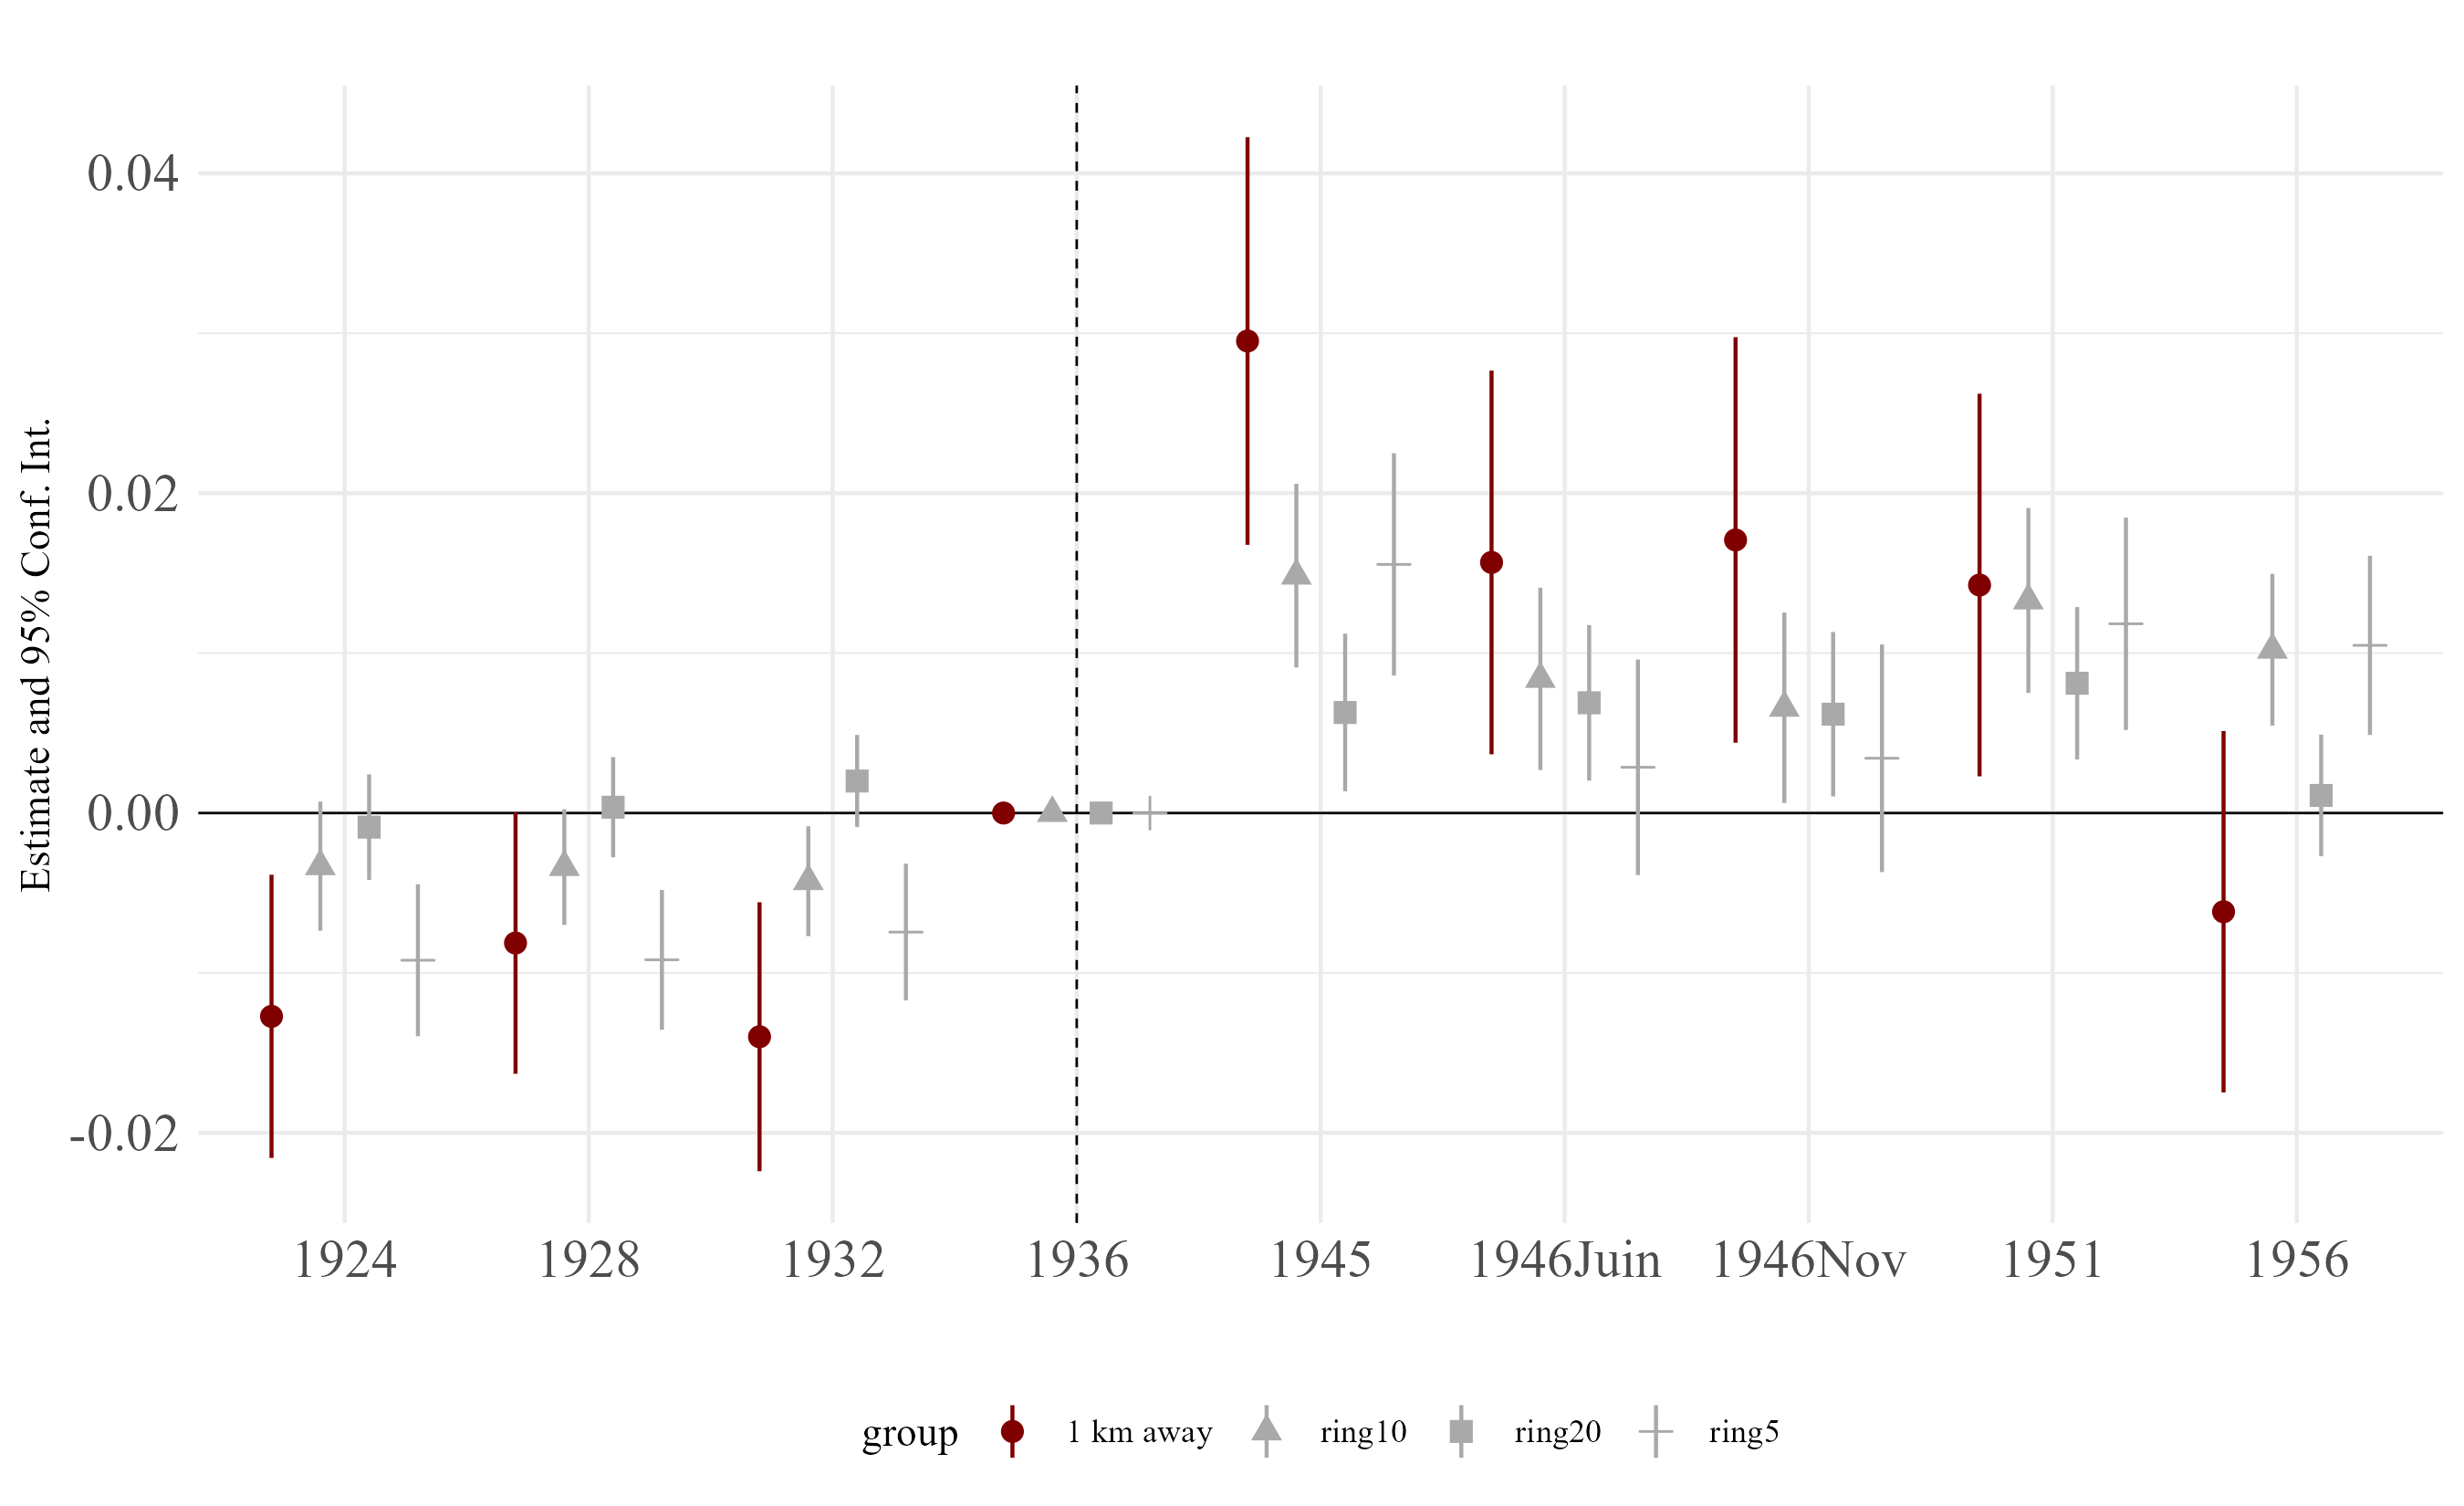
\includegraphics[width=0.8\linewidth]{figures/results/political/pvoixPCF_event_study.png}
  \label{fig:SFIO_all}
   \begin{minipage}{0.7\textwidth}
        \vspace{0.5em}
        {\footnotesize Notes: This graph reports the estimates from \cref{equation:political}, where the coefficient for each ring is estimated using municipalities located 20–40 km away as the control group. Error bars plot the interval confidence at 95\%. Standard errors are clustered at the municipality level.\par}
        \end{minipage}
\end{figure}


We argue that the political effect that we document depends on the size of the camps the local population are exposed to. The effects of refugees camps by the size of the camp are jointly estimated in the same regression. In \autoref{fig:PCF_SFIO_camps_sizes}, we show the ATT on the share of votes for the SFIO and the PCF within a buffer of 1 kilometre of exposure, depending on the size of the camps they are exposed as defined by the quartile in terms of refugees population\footnote{See \autoref{fig:bars_camps_sizes} for the definition of the quartiles.}. The exposure to a camps with a refugee population lower than 20 individuals does not have any significant effect on the vote for the communist party after the war, and is slight significant for the socialist party. Overall, we observe a positive correlation between the size of the camp population and both the magnitude and statistical significance of the effect that we measure. EVENT STUDIES IN THE ANNEX. 



\begin{figure}[h!]
  \centering
  \caption{Impact on the Share of Votes, per Size of Camps}
  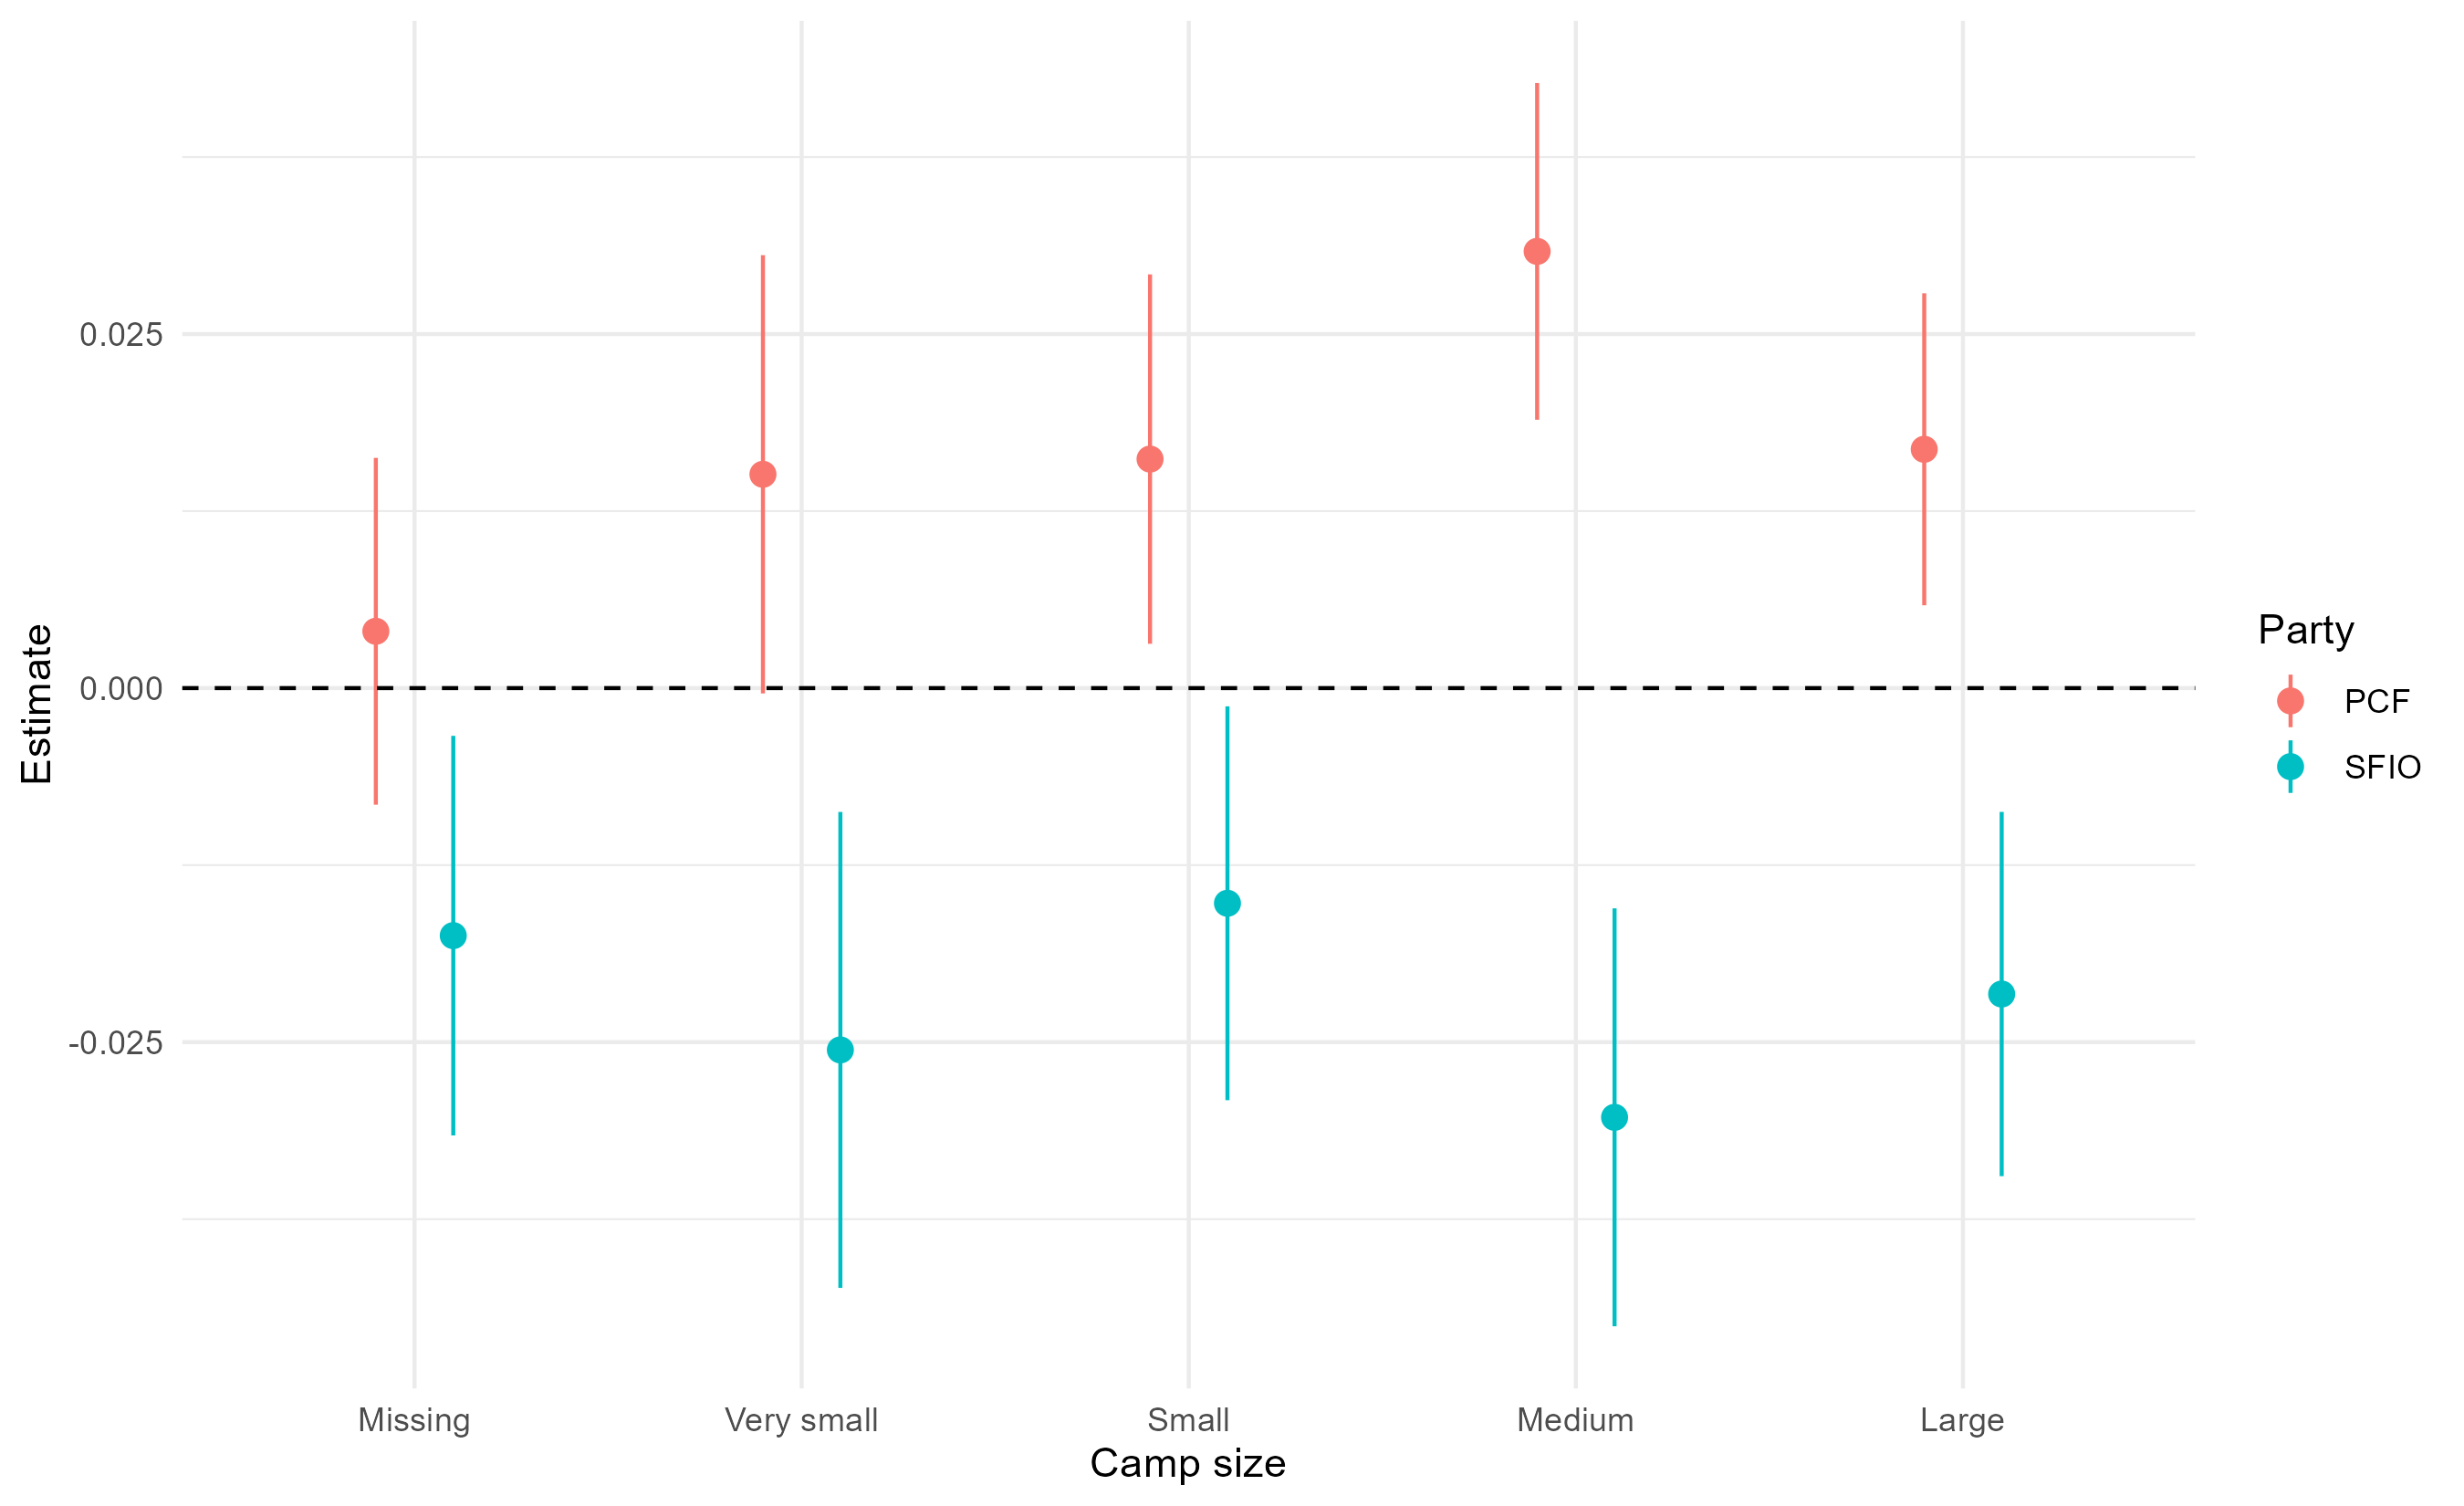
\includegraphics[width=0.8\linewidth]{figures/results/political/effect_size.png}
  \label{fig:PCF_SFIO_camps_sizes}
   \begin{minipage}{0.7\textwidth}
   \vspace{0.1in} 
        {\tiny This graph reports the jointly estimated average treatment effects of the different camps, by size, on vote shares for the Socialists (SFIO) and the Communists (PCF). The control municipalities are those within 20-40 km. The distribution of the population camps and their categorization per population quartiles is reported in \autoref{fig:bars_camps_sizes}.Error bars plot the interval confidence at 95\%. Standard errors are clustered at the department level.\par}
        \end{minipage}
\end{figure}



\subsection{Results in mobilization}


We now examine whether the effects differ across the political spectrum to explore political polarization and diffusion of ideas. We explore the relationship between the location of the camps and the resistance movement to explore the effect on the behaviour among a politically selective minority rather than population-wide responses. These measures reflect actions taken by individuals who were already highly engaged in political or civic life. Several organizations were especially active in mobilizing around the arrival of the Spanish refugees: the General Confederation of Labour (CGT), professional unions and cooperative federations. Members of these groups were more likely to interact directly with the Republican refugees. If ideas brought by the refugees diffused locally, politically active individuals are the ones most likely to internalize and act upon them. Any diffusion mechanism would therefore be expected to appear at the political extremes, where responses may diverge from those of the average voter.

%collaborators: and \Cref{fig:collabos} 
%in the case of resistance, whereas it remains significant up to 15 km for collaboration. This pattern cannot be explained by political selection in the siting of the camps. Instead, it aligns with increasing political polarization in municipalities closer to the camps. 

\Cref{fig:resistants} displays coefficient estimates by distance to the nearest refugee camp, with each point corresponding to a separate regression. The results indicate a positive association between proximity to a camp and resistance participation. This effect is concentrated within 3 km and disappears at larger distances. Within this radius, camp proximity is associated with an approximately 13\% increase in the expected number of individuals participating in the resistance, corresponding to about 1.5 additional individuals per municipality. This pattern is consistent with the results on the communist party, considering the links between the PCF and the resistance movement. 


\begin{figure}[htbp]
  \centering
    \caption{Effect of Refugee Camp Exposure on Resistance, by Distance}
  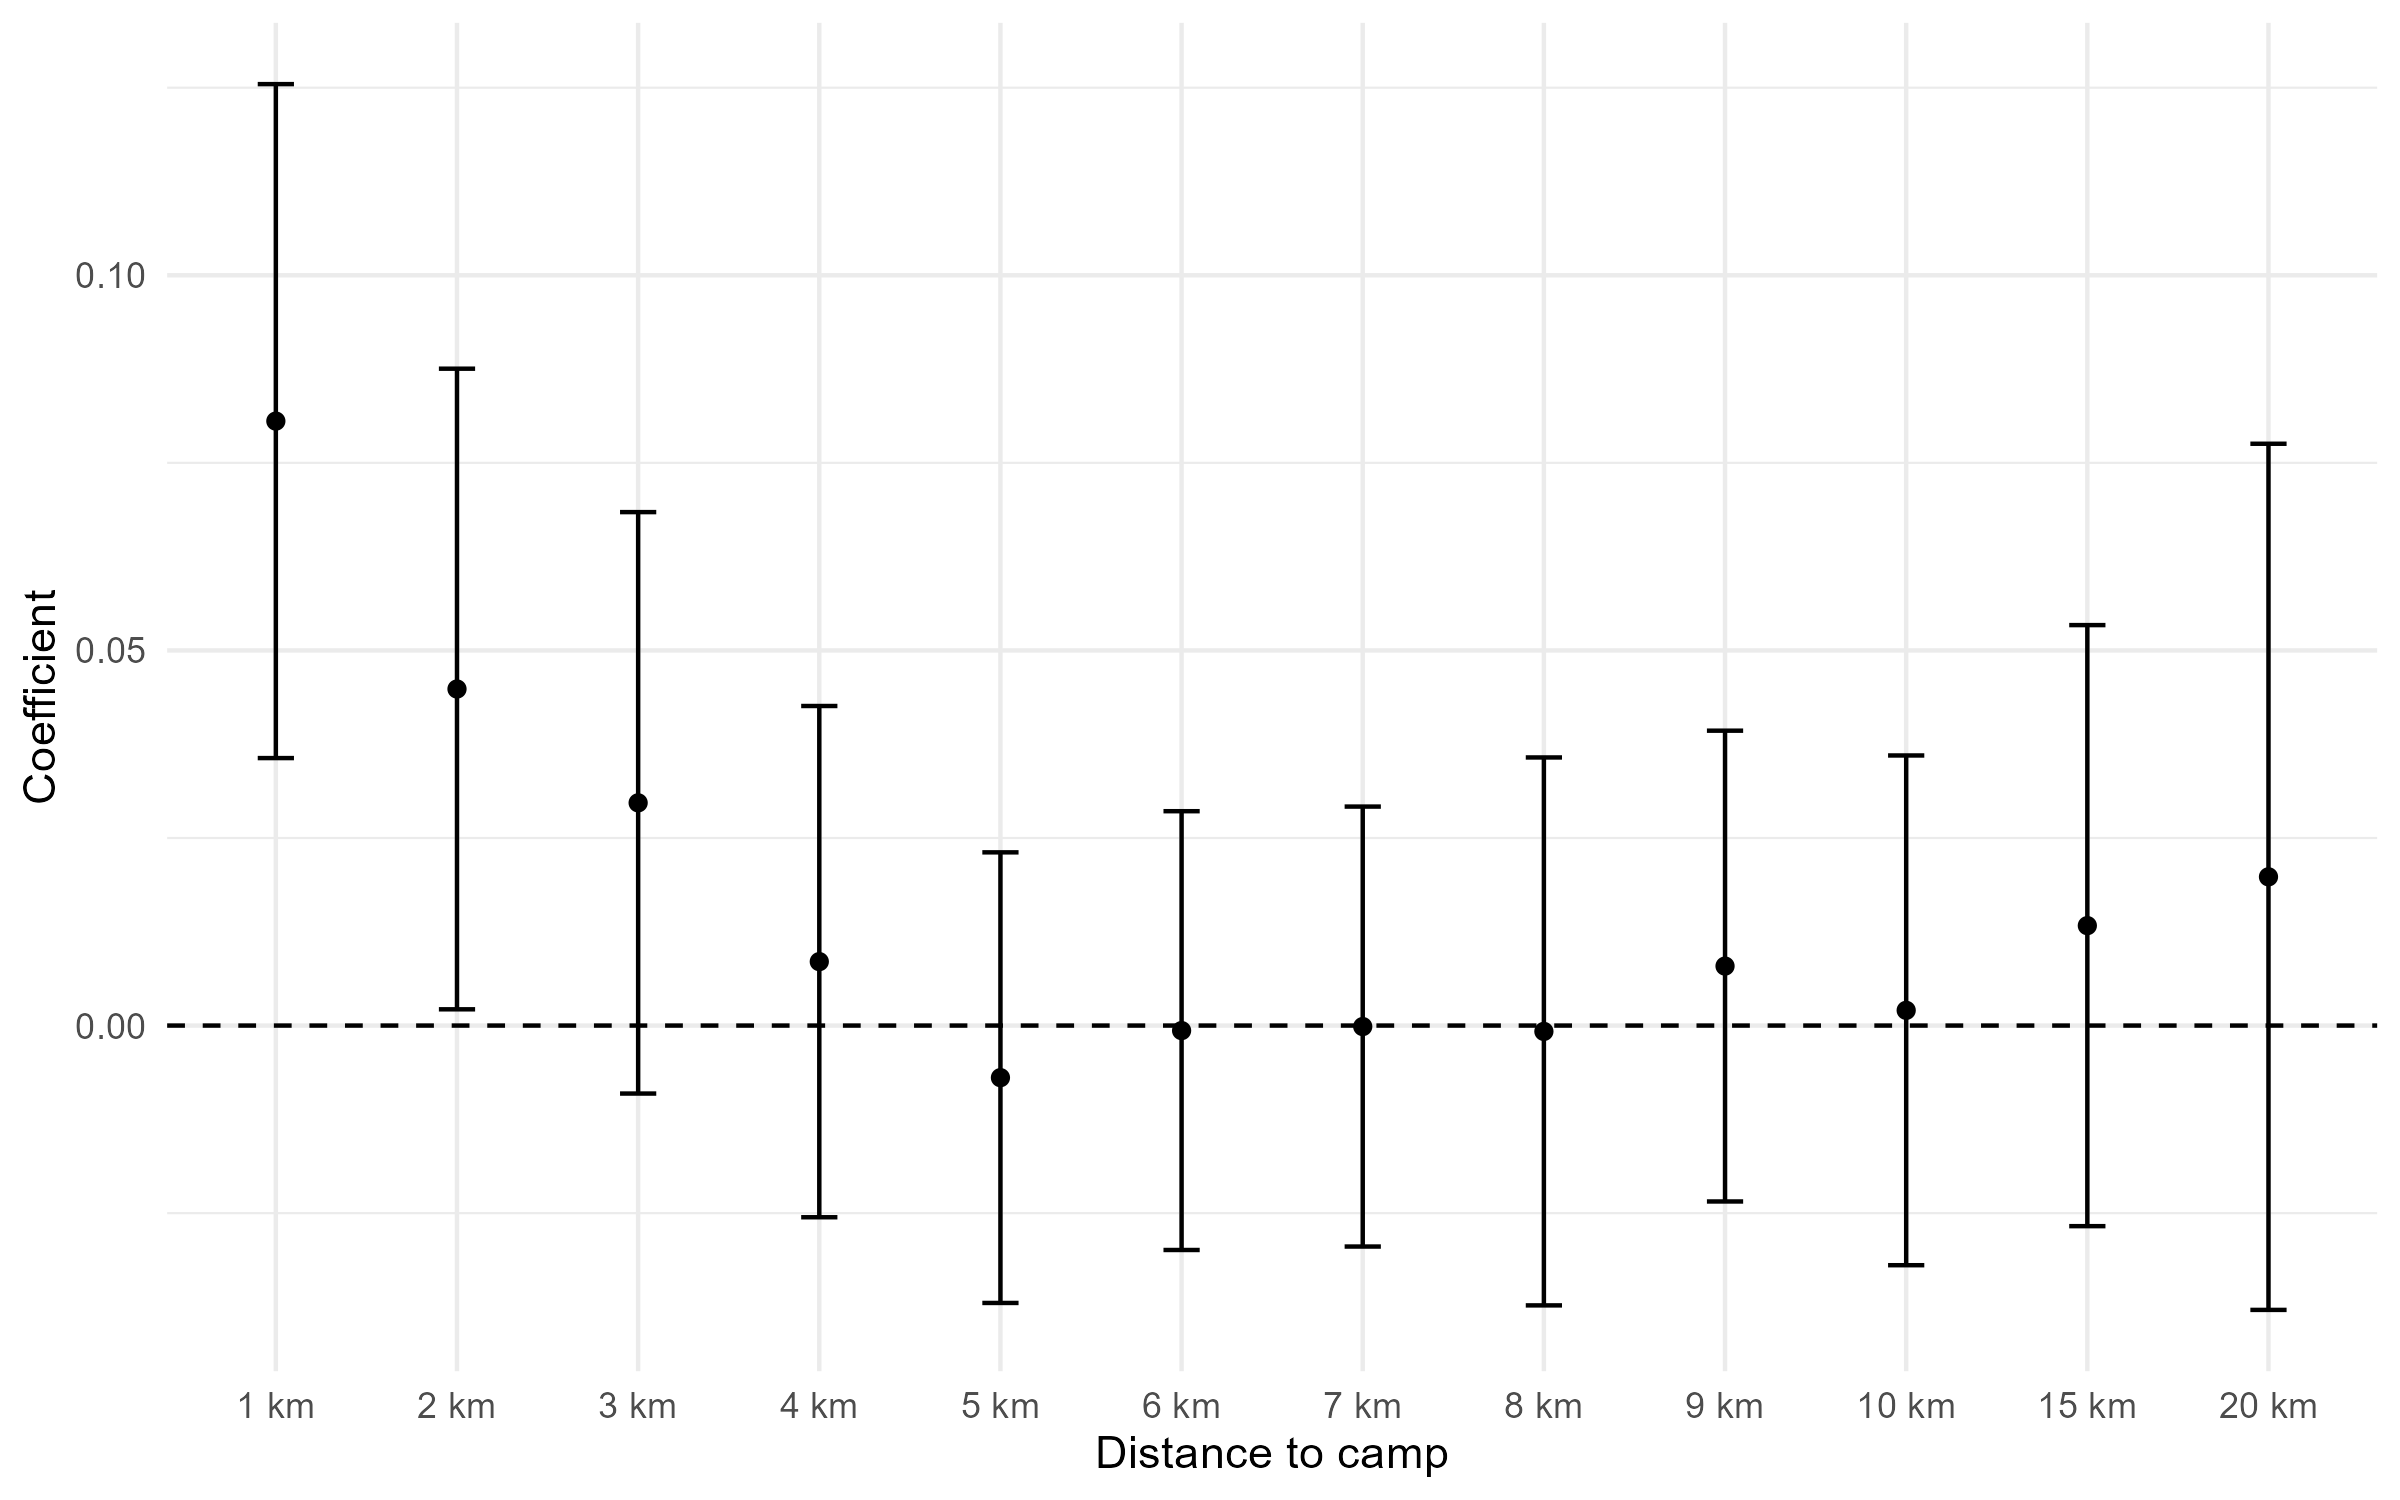
\includegraphics[width=0.8\linewidth]{figures/results/mobilisation/poisson_count_total.png}
  \label{fig:resistants}
   \begin{minipage}{0.8\textwidth}
        \vspace{0.1in} 
        {\footnotesize Notes: This graph reports the estimates of Poisson regressions on the number of resistants against Nazi Occupation. Error bars plot the interval confidence at 95\%. Standard errors are clustered to account for spatial correlation using \citet{conley_gmm_1999} (100 km). All specifications include region fixed effects and a set of controls—surname-based birthplace composition, altitude, mining activity, buildings per capita, average rainfall and the share of votes for the political parties of the 1936 legislative elections —and include a population offset.\par}
        \end{minipage}
\end{figure}

\begin{figure}[htbp]
  \centering
    \caption{Effect of Refugee Camp Exposure on Resistance, by size of the camp}
  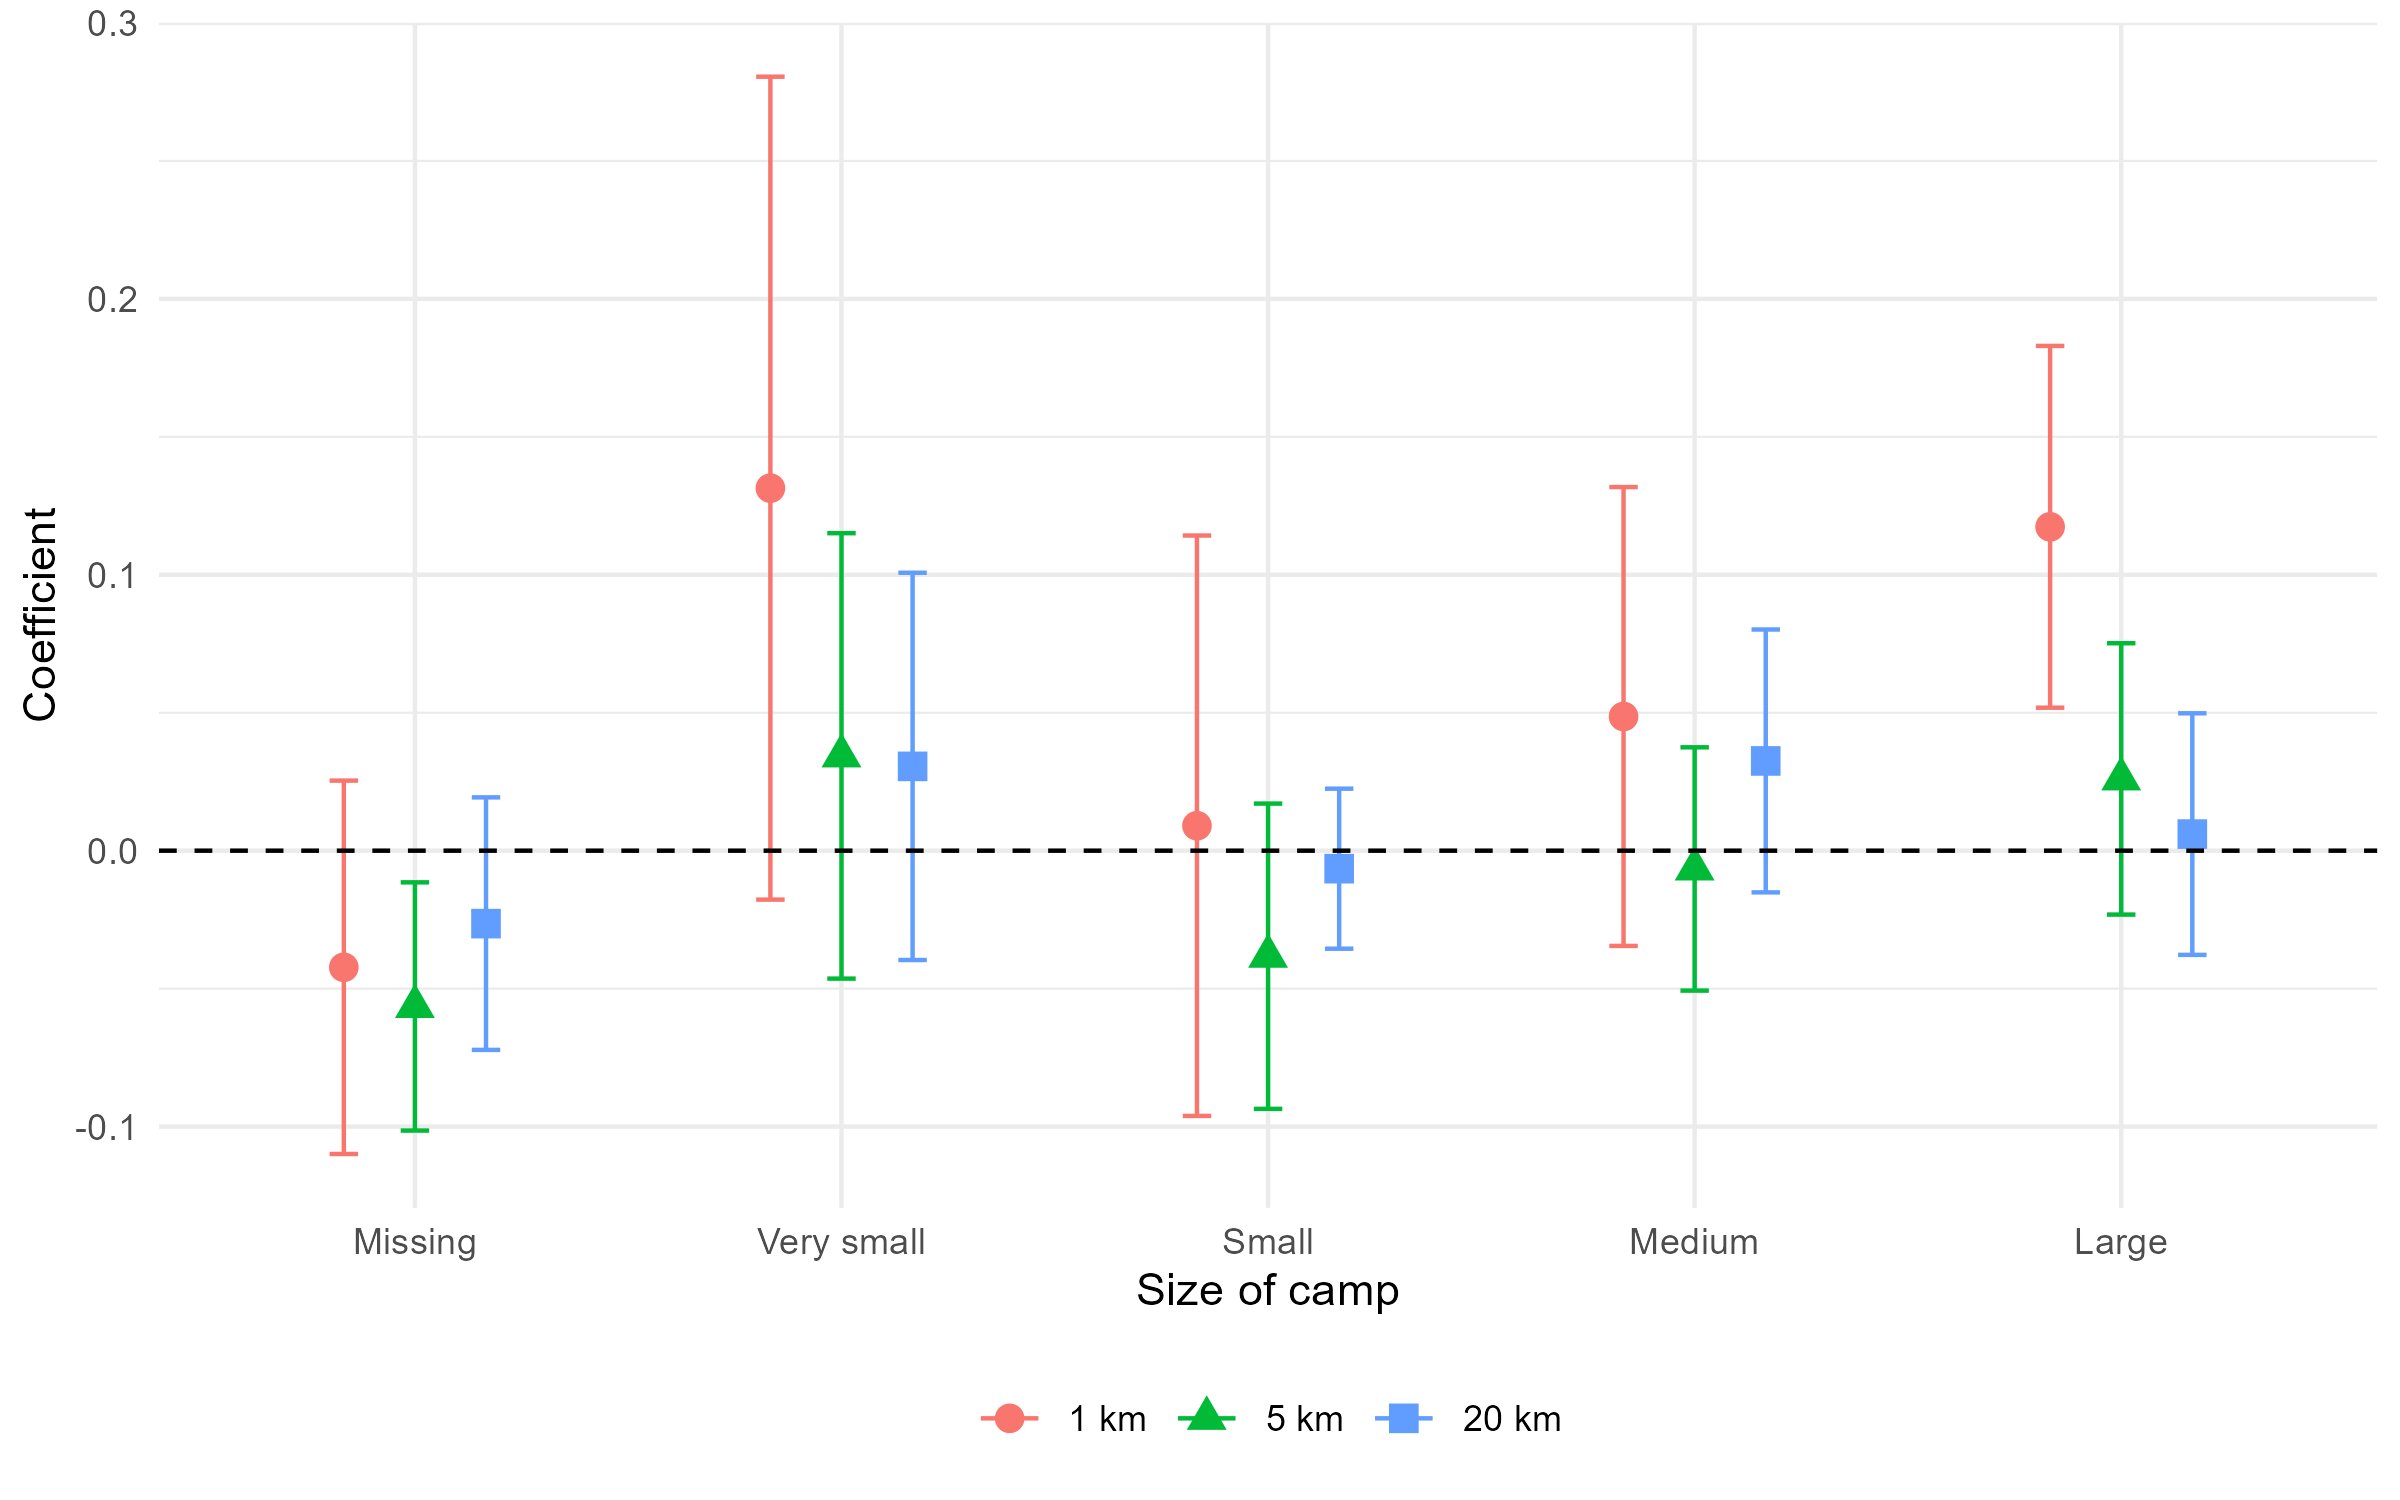
\includegraphics[width=0.8\linewidth]{figures/results/mobilisation/by_size_resistants.png}
  \label{fig:resistants}
   \begin{minipage}{0.8\textwidth}
        \vspace{0.1in} 
        {\footnotesize Notes: This graph reports the estimates of Poisson regressions on the number of resistants against Nazi Occupation. Error bars plot the interval confidence at 95\%. Standard errors are clustered to account for spatial correlation using \citet{conley_gmm_1999} (100 km). All specifications include region fixed effects and a set of controls—surname-based birthplace composition, altitude, mining activity, buildings per capita, average rainfall and the share of votes for the political parties of the 1936 legislative elections —and include a population offset.\par}
        \end{minipage}
\end{figure}


We further explore the political mobilization impact of exposure to Spanish refugees by examining its effect on the creation of associations. To assess this, we classify associations based on their names and descriptions of activities as listed in the Registre National des Associations. Our main results regarding these outcomes are presented in \autoref{tab:att_associations_large_medium}\footnote{The corresponding event study plots are available in \autoref{apdx:}}. Specifically, we identify four types of associations of interest: associations related to Migrants and Refugees, Solidarity associations, Left-wing and Union associations, and those focused on military and Resistance activities\footnote{We determine whether an association belongs to one of these categories based on a list of key words that unequivocally indicate the type of activity. These lists of key words are available in the Appendix.}. We then apply the same empirical strategies as before at the canton level, comparing localities that have welcomed large and medium camps of refugees with those that have not. Our findings show a positive effect on the creation of associations after the Retirada for associations related to refugee support, as well as for unions and left-wing groups. As a placebo, we also demonstrate that other types of associations, such as sports and religious groups, do not exhibit the same effects (see columns (5) and (6), showing results for these types of associations). While this effect aligns with the political mobilization observed through voting patterns post-WWII, as well as the backlash against the Socialist Party and the Radicals, our results also provide evidence of the type of interactions that may have contributed to the rise in both Resistance behaviour and the transmission of values.



\begin{table}[h!]
    \centering
    \caption{Association Creations, by Type, pre- and post- WWII}
    \resizebox{\textwidth}{!}{
\begingroup
\centering
\begin{tabular}{lcccccc}
   \toprule
                                     & Refugees      & Solidarity    & Unions/Left-wing & Resistance     & Sport         & Religion\\  
                                     & (1)           & (2)           & (3)              & (4)            & (5)           & (6)\\  
   \midrule 
   Large/Medium $\times$ civil war   & 0.5597        & 0.1689        & 0.1660$^{**}$    & -0.0010        & 0.0825        & -0.0093\\   
                                     & (0.4194)      & (0.1915)      & (0.0751)         & (0.0954)       & (0.0551)      & (0.2184)\\   
   Large/Medium $\times$ 1939     & 0.2568        & -0.3469       & 0.0579           & 0.1021         & 0.0289        & 0.2077\\   
                                     & (0.7100)      & (0.2655)      & (0.1417)         & (0.1712)       & (0.0972)      & (0.3350)\\   
   Large/Medium $\times$ 1940        & 1.489$^{**}$  & 0.5578        & 0.5441$^{**}$    & 0.7235$^{***}$ & 0.0290        & 0.2425\\   
                                     & (0.6344)      & (0.3633)      & (0.2116)         & (0.1940)       & (0.1778)      & (0.4230)\\   
   Large/Medium $\times$ 1944        & 1.035         & 0.7301        & 0.7710$^{***}$   & 0.0907         & 0.0196        & -0.3063\\   
                                     & (0.6546)      & (0.4610)      & (0.2701)         & (0.2330)       & (0.1506)      & (0.4596)\\   
   Large/Medium $\times$ 1945        & 1.266$^{**}$  & 0.0219        & 0.0799           & 0.3513$^{***}$ & 0.0144        & 0.0247\\   
                                     & (0.5680)      & (0.2097)      & (0.1947)         & (0.1144)       & (0.0707)      & (0.2454)\\   
   Large/Medium $\times$ 1946        & 0.9083        & 0.2943        & 0.1716           & 0.1340         & 0.0606        & -0.3760\\   
                                     & (0.6377)      & (0.2263)      & (0.1096)         & (0.1285)       & (0.0722)      & (0.2859)\\   
   Large/Medium $\times$ 1947-1950   & 0.9719$^{**}$ & 0.2175        & -0.0698          & 0.0864         & 0.0209        & 0.0600\\   
                                     & (0.4870)      & (0.1694)      & (0.0771)         & (0.1057)       & (0.0537)      & (0.1773)\\   
   Controls                          & $\checkmark$  & $\checkmark$  & $\checkmark$     & $\checkmark$   & $\checkmark$  & $\checkmark$\\   
    \\
   Observations                      & 1,946         & 10,067        & 23,622           & 20,738         & 29,564        & 9,156\\  
   Squared Correlation               & 0.70419       & 0.71786       & 0.76483          & 0.74927        & 0.85439       & 0.67070\\  
   Pseudo R$^2$                      & 0.32031       & 0.35288       & 0.41897          & 0.37466        & 0.46583       & 0.34794\\  
   BIC                               & 9,323.1       & 37,367.1      & 82,164.3         & 70,691.1       & 119,750.8     & 34,014.4\\  
    \\
   canton fixed effects              & $\checkmark$  & $\checkmark$  & $\checkmark$     & $\checkmark$   & $\checkmark$  & $\checkmark$\\   
   arrondissement-year fixed effects & $\checkmark$  & $\checkmark$  & $\checkmark$     & $\checkmark$   & $\checkmark$  & $\checkmark$\\   
   \bottomrule
\end{tabular}
\par\endgroup


}
    \label{tab:att_associations_large_medium}
    \par
        \begin{minipage}{\textwidth}
        \vspace{0.5em}
            \footnotesize
            Note: The table above reports coefficient of the Poisson estimates difference-in-differences regression at the canton level, comparing canton that have welcomed refugees with the ones that have not. Here treatment is only taking into account medium-size and large-size camps. To ensure comparability, control only takes into account the canton that are within a buffer of 40 km around this types of camps. We control for the total population of the canton per year as well as for the left-wing last election results. Our main specification takes into account canton fixed effects and arrondissement $\times$ year fixed effect. *** p$<$0.01, ** p$<$0.05, * p$<$0.1.
        \end{minipage}
\end{table}